\documentclass[conference, a4paper]{IEEEtran}

\usepackage{graphicx}
\usepackage[style=ieee]{biblatex}
\addbibresource{bibliography.bib}

\title{A hierarchical, distributed MQTT-like protocol}

\author{\IEEEauthorblockN{Alexander Thomas}
\IEEEauthorblockA{School of Electronics and Computer Science\\
University of Southampton\\
Email: CONFIDENTIAL\\
Student ID: CONFIDENTIAL}
}

\begin{document}
    \maketitle
    \begin{abstract}
        MQTT is a networking protocol commonly used in the Internet of Things (IoT), which supports a `publish-subscribe' method of communication in which messages are grouped by hierarchical `topics'.
        In simple MQTT deployments there is a bottleneck in the system, because of reliance on a single `broker' device which all messages pass through, which may cause problems in large systems.
        There are several existing systems which attempt to mitigate this, which generally rely on exploiting multi-core processors, or using several brokers and duplicating messages between them as necessary.
        This report documents an approach to designing a scalable MQTT-like broker which avoids duplicating messages by limiting the jurisdiction of each broker to a subtree of the topic hierarchy, without overlap.
    \end{abstract}

    \section{Introduction}
        MQTT is a networking protocol which facilitates a publish-subscribe messaging model, similar to the observer design pattern in object-oriented programming but over a network.
        Messages are grouped by `topics', which have a hierarchical structure, and subscribers are able to subscribe to whole sub-hierarchies of the system through wildcards.
        All of this functionality is achieved through an MQTT `broker', which is a piece of software which receives published messages and distributes them to the appropriate subscribers.


        This architecture presents a clear bottleneck at the broker, as all of the messages in the system must pass through this single device.
        This could cause a problem in systems that push a large amount of data through the system, for example in a security camera system the multiple video streams could be too much for a single broker to cope with.
        There are a number of existing systems aimed at improving the scalability of the broker.
        Spreading the role of the broker across multiple servers is a common approach, however many commercially available systems and those documented in the literature may require multiple of these brokers to distribute any given message, meaning the message must be relayed and duplicated across each of these brokers.


        In this report, an approach is documented through which each broker is allocated some subtree of the topic hierarchy and manages only messages in that subtree, exclusively from other brokers.
        The system is built on a custom protocol similar to MQTT, but based on UDP because it is not possible to connect with the multiple brokers required with a single persistent connection (i.e. via TCP).
        This design avoids the duplication of messages between brokers, and therefore it is hypothesized that the system could allow more scalable message broker systems.

    \section{Related Work}
        There are two main approaches taken in the literature to improving the scalability of MQTT brokers.
        The first of these is to exploit the multiple cores available in modern processors.
        MuMQ\autocite{wiriyang17} is an example of this, spreading the task of handling each incoming TCP connection between several CPU threads.
        In addition to this, a user-level TCP/IP stack, mTCP is used to reduce the overhead of the kernel TCP/IP stack.
        This system is documented outperforming Mosquitto, a popular MQTT broker implementation, by 538\%.

        
        The second common approach to improving scalability is through `clustering'.
        This is a technique in which several brokers are used in the system, with the goal of reducing the workload at any single broker.
        Some of these systems allow new brokers to be dynamically added and removed from the system, meaning that new broker systems could be started or shut down based on demand, for example through Infrastructure-as-a-Service providers\autocite{koziolek20}.


        Jutadhamakorn et al.\autocite{jutadhamakorn17} present an approach to this using NGINX as a load balancer to distribute subscriptions to a cluster of MQTT brokers running Mosquitto\autocite{mosquitto}.
        In this system, messages are published to all of the mosquitto nodes by a `middle-man' system which communicates with the actual clients.

        
        An analysis of the performance of several commercial clustered MQTT brokers is provided in \autocite{koziolek20}.
        EMQX\autocite{emqx} was found to perform best from the 3 systems tested, with a throughput of 28,000 messages per second.
        This is a clustered MQTT broker based on erlang, and as with other clustered MQTT brokers, it must distribute messages between the broker nodes if a subscriber is connected to a different node from that at which the message arrived.

    \section{Design}
        The goal with this project is to produce a distributed broker where it is guaranteed that when a message arrives at one of the nodes, that node is able to reach all of the clients with subscriptions for that message without having to consult with other nodes, or relay the message to other nodes.
        With standard MQTT, this is not possible; when a client connects to the broker, it expects to form a single, continuous TCP connection with the broker.
        As has been shown in the literature, the node to which this connection is made can be selected through `middle-man' systems such as load-balancers \autocite{jutadhamakorn17}, however MQTT allows subscription to multiple topics through the use of wildcards (i.e. `+' and `*'), meaning a single subscription may involve multiple nodes depending on how topics are allocated between nodes, if there is any topic segregation between brokers at all.


        Because of this, my solution uses UDP instead of TCP, because it is connectionless.
        After sending its subscription to the broker, the client can receive published messages as a UDP packet from any node in the system without issue, whereas with TCP it would only be able to receive them from the node to which it originally connected.
        In this system, subscriptions are not represented by open TCP connections, but by records stored in each of the involved broker nodes.


        \begin{figure*}[t]
            \centering
            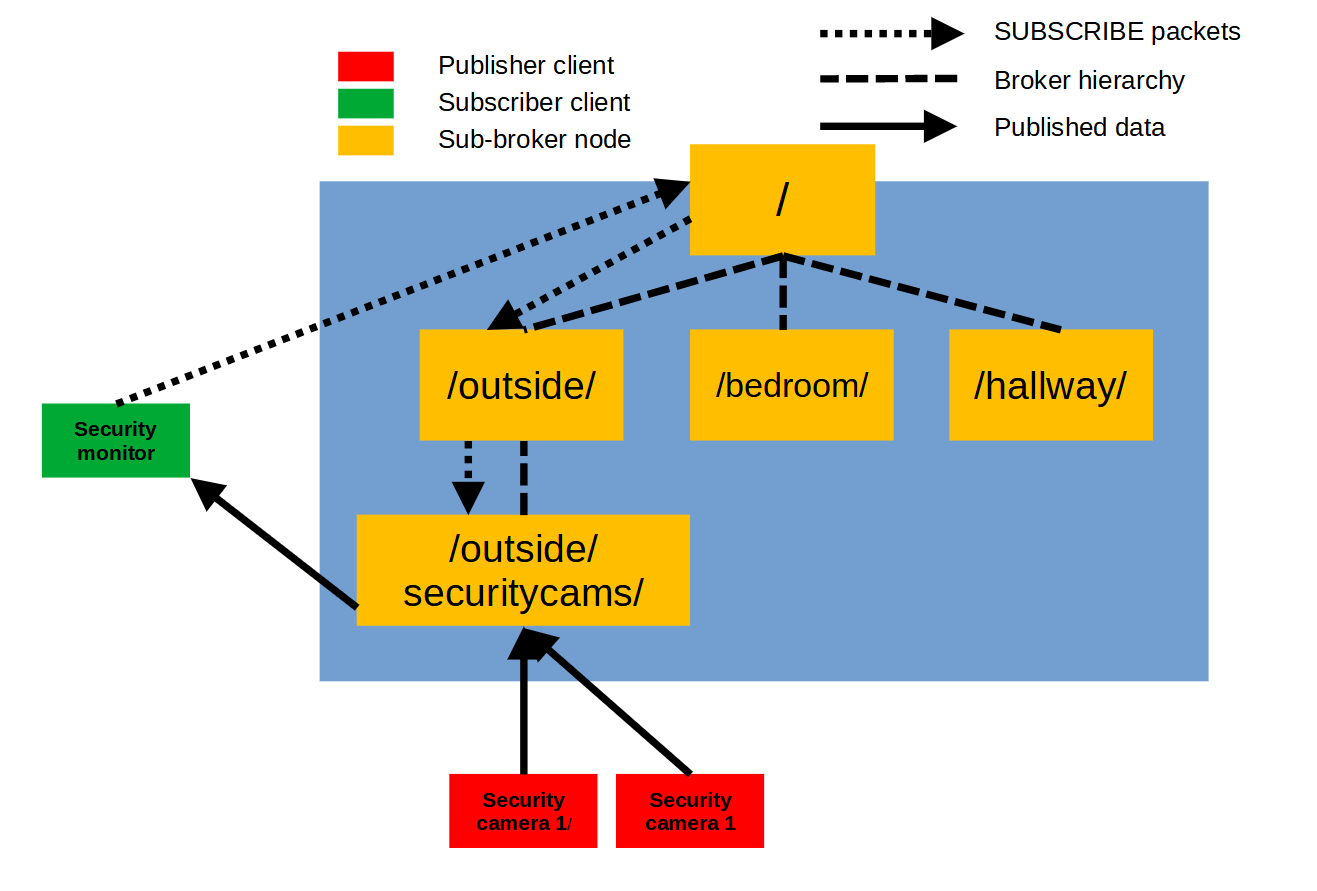
\includegraphics[width=0.9\textwidth]{fig1.png} 
            \caption{An example topic hierarchy with a security monitor subscribing to one of the security cameras. The flow of the \texttt{SUBSCRIBE} packet through the system is shown; only the \texttt{/outside/securitycams/} nodes stores the subscription.}
            \label{fig:one}
        \end{figure*}
        
        Each node comprising the broker is responsible for a specific subtree of the topic hierarchy, with a `root' node forming the main endpoint of the system.
        For example, in a home IoT system, with subtopics for several rooms, there could be a separate sub-broker set up for each of these rooms, which would be responsible for all of the sub-subtopics in the room, i.e. a sub-broker would be set up for subtree `/kitchen/', and this would handle messages on /kitchen/oven/, /kitchen/lights/, and /kitchen/refrigerator/, etc.
        These sub-brokers are able to `join' a parent broker, which then delegates responsibility for that part of the topic tree to the new sub-broker (meaning in the example system above there would need to be a `root' broker (i.e. with subtree `/') in addition to the sub-brokers for each room).
        The system could also be operated with only the root broker, in which case this broker is responsible for all of the communication in the system, as with conventional MQTT brokers.


        In order to find the appropriate broker to publish messages to, a `publisher' client `resolves' the appropriate node through a process somewhat similar to a DNS lookup.
        A connection request is sent to the root node, which then passes the request down the tree until it reaches the node with jurisdiction for the topic the client has requested.
        This node then responds to the client, providing its IP address and UDP port, to which the client can now simply send messages.


        Subscriptions are handled in a similar way; a request is sent to the root broker, and then propagates through the appropriate subtrees of the system.
        Nodes with jurisdiction over all of part of (i.e. wildcards) the subscription store the subscription (i.e. the requested topic and the client's IP and UDP port) before passing it down the tree if necessary.
        An example of this process is shown in figure \ref{fig:one}.


        This does mean that there is some communication required between the nodes in the system, however crucially there is never the requirement for actual data messages to be duplicated between brokers, only `control' messages (i.e. sub-broker join requests, subscriptions, and publisher connection requests).
        It is expected that the quantity of these will be considerably lower than that of data publishes, so it is hoped that this represents less overhead than other systems where multiple nodes have a role in the distribution of a single message.


    \section{Implementation}
        A broker is implemented in C++, using the socket API to send and receive UDP packets.
        To demonstrate the system, a program which can publish strings from stdin to a topic, and a program which subscribes to a topic and prints received messages have also been written.
        At present, brokers and nodes use only a single thread for simplicity, as the system is only intended as a proof of concept.
        Real-world systems would likely provide much higher throughput per node with a multi-threaded implementation.


        The protocol is implemented using Protocol Buffers\autocite{protobuf}, a serialisation library which stores the data comprising each packet in the protocol in a compact, binary form for transmission in a UDP packet.
        This library also helps to avoid issues relating to compatibility between systems, such as endianness and padding due to system word length.


        The protocol is comprised of 6 message formats:
        \begin{itemize}
            \item \texttt{PUBCONNECT}: Sent to the root broker by publishers to establish the sub-broker responsible for the topic to which it would like to publish.
            \item \texttt{PUBACCEPT}: Sent from the appropriate sub-broker to a publisher to signify that it is able to accept messages on the requested topic.
            \item \texttt{PUBLISH}: Sent by a client to publish new data to a topic, and relayed by the broker to subscribing clients.
            \item \texttt{PUBACK}: Response to a \texttt{PUBLISH} from the broker to signify distribution of the message has been completed, or that the publication failed, e.g. due to a new sub-broker taking over responsibility for the topic.
            \item \texttt{SUBSCRIBE}: Sent by a client to the root broker to subscribe to a topic.
            \item \texttt{JOIN}: Sent from a sub-broker to its parent, requesting to take over control of part of the topic hierarchy.
        \end{itemize}
        These packet formats are wrapped in another protobuf message format using \texttt{oneof}, which allows protobuf to distinguish between them from the packet arriving over the network.


        C++ standard library containers are used to store sub-brokers and subscriptions in the broker program.
        An \texttt{std::unordered\_map} with topic as key and IP address as value is used for sub-brokers (for fast lookup and comparison with incoming subscriptions), and an \texttt{std::vector} is used for subscriptions (holding the subscribed topic and the address of the subscriber).

    \section{Conclusions and Future Work}
        The system works as initially planned, and it has been shown that this approach effectively spreads the majority of the tasks of the broker between the nodes, especially if traffic is well distributed across topics.
        It has not been possible to establish how the system compares with other commercially available MQTT and message broker systems, as only a simple proof of concept broker node was implemented, which does not use techniques that have been shown to drastically improve performance (e.g. multithreading), and does not support the full feature set of MQTT.
        Following the proof of the concept demonstrated in this project, It would be helpful to implement a more robust message broker node using this approach, which could then be compared against other available message broker systems.


    \printbibliography
\end{document}
